\documentclass{article}
\usepackage[paperwidth=20cm, paperheight=6cm, margin = 0cm, top=0.5cm]{geometry}
\usepackage{amsmath}


\usepackage{pgf}
\usepackage{tikz}


\usetikzlibrary{arrows,automata}

\tikzstyle{source}  = [draw,circle,fill=black,thick,inner sep=0mm,minimum size=2mm]

\renewcommand{\vec}[1]{\boldsymbol{#1}}

\begin{document}
\begin{center}
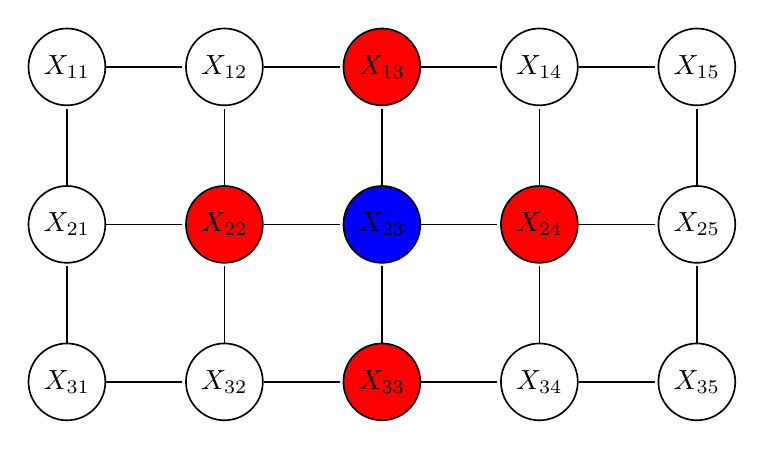
\begin{tikzpicture}[-,>=stealth',shorten >=1pt,auto,node distance=2cm,semithick]
                    
\node[state] (X1)               {$X_{31}$}; 
\node[state] (X2) [right of=X1] {$X_{32}$};                   
\node[state, fill=red] (X3) [right of=X2] {$X_{33}$};                   
\node[state] (X4) [right of=X3] {$X_{34}$};                   
\node[state] (X5) [right of=X4] {$X_{35}$};                   

\node[state] (Y1) [above of=X1] {$X_{21}$}; 
\node[state, fill=red]  (Y2) [above of=X2] {$X_{22}$}; 
\node[state, fill=blue] (Y3) [above of=X3] {$X_{23}$}; 
\node[state, fill=red]  (Y4) [above of=X4] {$X_{24}$}; 
\node[state] (Y5) [above of=X5] {$X_{25}$}; 

\node[state] (Z1) [above of=Y1] {$X_{11}$}; 
\node[state] (Z2) [above of=Y2] {$X_{12}$}; 
\node[state, fill=red] (Z3) [above of=Y3] {$X_{13}$}; 
\node[state] (Z4) [above of=Y4] {$X_{14}$}; 
\node[state] (Z5) [above of=Y5] {$X_{15}$}; 

	
\path
	(X1) edge (X2)
	(X2) edge (X3)
	(X3) edge (X4)
	(X4) edge (X5);
\path
	(Y1) edge (Y2)
	(Y2) edge (Y3)
	(Y3) edge (Y4)
	(Y4) edge (Y5);
\path
	(Z1) edge (Z2)
	(Z2) edge (Z3)
	(Z3) edge (Z4)
	(Z4) edge (Z5);

\path	
	(X1) edge (Y1)
	(X2) edge (Y2)
	(X3) edge (Y3)
	(X4) edge (Y4)
	(X5) edge (Y5);
\path	
	(Y1) edge (Z1)
	(Y2) edge (Z2)
	(Y3) edge (Z3)
	(Y4) edge (Z4)
	(Y5) edge (Z5);


\path	
	(Y1) edge (Z1)
	(Y2) edge (Z2)
	(Y3) edge (Z3)
	(Y4) edge (Z4)
	(Y5) edge (Z5);


\end{tikzpicture}
\end{center}

\end{document}
